\documentclass[12pt]{article}

\usepackage[utf8]{inputenc}
\usepackage{latexsym,amsfonts,amssymb,amsthm,amsmath}
\usepackage{float}

\setlength{\parindent}{0in}
\setlength{\oddsidemargin}{0in}
\setlength{\textwidth}{6.5in}
\setlength{\textheight}{8.8in}
\setlength{\topmargin}{0in}
\setlength{\headheight}{18pt}
\usepackage{graphicx}
\usepackage{tikz}

\usepackage{hyperref}
\hypersetup{
    colorlinks=true,
    linkcolor=blue,
    filecolor=magenta,      
    urlcolor=cyan,
    pdftitle={Overleaf Example},
    pdfpagemode=FullScreen,
}

\urlstyle{same}

\usepackage{caption}
\DeclareCaptionFormat{citation}{%
  \ifx\captioncitation\relax\relax\else
    \captioncitation\par
  \fi
  #1#2#3\par}
\newcommand*\setcaptioncitation[1]{\def\captioncitation{\textit{Source:}~#1}}
\let\captioncitation\relax
\captionsetup{format=citation,justification=centering}


\title{MATH1034OL1 Pre-Calculus Mathematics Notes from Section 2.5 (Friday)}
\author{Elijah Renner}

\begin{document}

\maketitle

\vspace{0.5in}

\tableofcontents

\section{Inverse Functions}

\subsection{Finding Inverses}
Given a function \(f(x)\), we denote its inverse as \(f^{-1}(x).\) To find the inverse of \(f(x)\):\\

\begin{enumerate}
  \item Replace \(f(x)\) with \(y\).
  \item Switch \(y\) and \(x\).
  \item Solve for \(y\).
  \item Replace \(y\) with \(f^{-1}(x)\)
\end{enumerate}

Here's an example:\\

Problem: Let \(f(x)=x^2+3\). Find \(f^{-1}(x)\).\\

Replace \(f(x)\) with \(y\): \(f(x)=x^2+3\implies y=x^2+3\)\\

Switch \(x\) and \(y\): \(y=x^2+3\implies x=y^2+3\)\\

Solve for \(y\): \(x=y^2+3\implies y^2=x-3 \implies y=\sqrt{x-3}\)\\

Replace \(y\) with \(f^{-1}(x)\): \(f^{-1}(x)=\sqrt{x-3}\)\\

Now we know \(f^{-1}(x)=\sqrt{x-3}\).\\

\subsection{Properties of Inverses}

A cool property of inverse functions is that \(f(x)\) and \(f^{-1}(x)\) reflect over the line \(y=x\):\\

\begin{figure}[H]
	\centering
	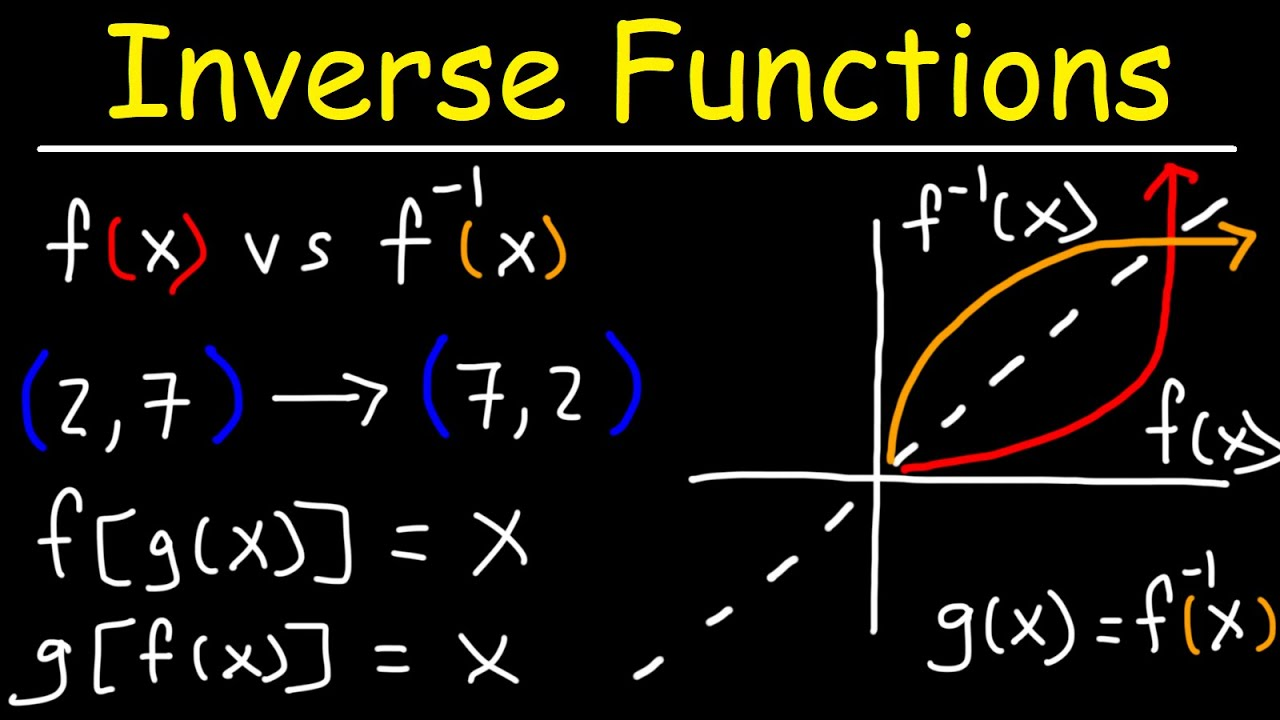
\includegraphics[scale=0.2]{maxresdefault.jpg}
	\caption{Credit: \url{https://youtu.be/TN4ybFiuV3k}}
\end{figure}

This makes sense because we are switching \(x\) and \(y\).\\

Another property of \(f^{-1}\) is that its domain and range are the range and domain respectfully of \(f\). More formally:\\

\(\text{domain}(f)=\text{range}(f^{-1})\)\\

\(\text{range}(f)=\text{domain}(f^{-1})\)\\

\section{Factoring Higher-Degree Polynomials}

Let's suppose we have the equation \(8x^3+x+9\)=0. The left side isn't easily factorable and can't be plugged into the quadratic formula. Instead, we can find the possible rational zeros of the expression.\\

Let \(f(x)=a_nx^n+a_{n-1}x^{n-1}+...+a_2x^2+a_1x+a_0\) where  \(a\) are integers. Here,\\

\[\text{possible rational zeros}=\frac{\text{factors of }a_0\text{ (last term)}}{\text{factors of }a_n\text{(first term)}}\]

Hence, the possible rational zeroes of \(8x^3+x+9\) are \(\pm\frac{1,3,9}{1,2,4,8}=\pm\frac{1}{8},\pm\frac{1}{4}, \pm\frac{3}{8},\pm\frac{1}{2}, \pm\frac{3}{4},\pm1, \pm\frac{9}{8},\)

\(\pm\frac{3}{2}, \pm\frac{9}{4}, \pm\frac{9}{2},\pm3, \pm9\).\\


Personally, I like to start with integers. We can manually plug possible rational zeros in as \(x\). However, there's a trick to quickly evaluate polynomials at a certain value \(x\). This isn't easily explained in writing, so here's a helpful video from \href{https://www.youtube.com/watch?app=desktop&v=FxHWoUOq2iQ}{the Organic Chemistry tutor}. \\

Just remember that if \(f(a)=0\) than \((x-a)\) is a factor of \(f\).\\

\section{Midterm Concepts}

If you study these, you will do well on the midterm exam:

\begin{enumerate}
	\item Converting between degrees and radians
	\item Determining reference angles
	\item All Students Take Calculus
	\item Unit Circle \((x,y)=(\cos,\sin)\); \(\sec=\frac{1}{x}\), \(\csc\frac{1}{y}\); \(\tan=\frac{\sin}{\cos}=\frac{y}{x}\); \(\cot=\frac{\cos}{\sin}=\frac{x}{y}\)
	\item 30-60-90 triangle properties
	\item 45-45-90 triangle properties
	\item Trigonometric functions in terms of the sides of an angle:
		\[
		\tan \theta = \frac{\text{opp}}{\text{adj}}
		\]
		
		\[
		\sin \theta = \frac{\text{opp}}{\text{hyp}}
		\]
		
		\[
		\cos \theta = \frac{\text{adj}}{\text{hyp}}
		\]
		
		\[
		\cot \theta = \frac{\text{adj}}{\text{opp}}
		\]
		
		\[
		\csc \theta = \frac{\text{hyp}}{\text{opp}}
		\]
		
		\[
		\sec \theta = \frac{\text{hyp}}{\text{adj}}
		\]
	\item Composing functions and function operations
	\item Inverse functions
	\item Solving high degree polynomials and the rational zero theorem
	\item Equations of circles
\end{enumerate}




\end{document}
